% Created by tikzDevice version 0.11 on 2018-09-24 10:56:58
% !TEX encoding = UTF-8 Unicode
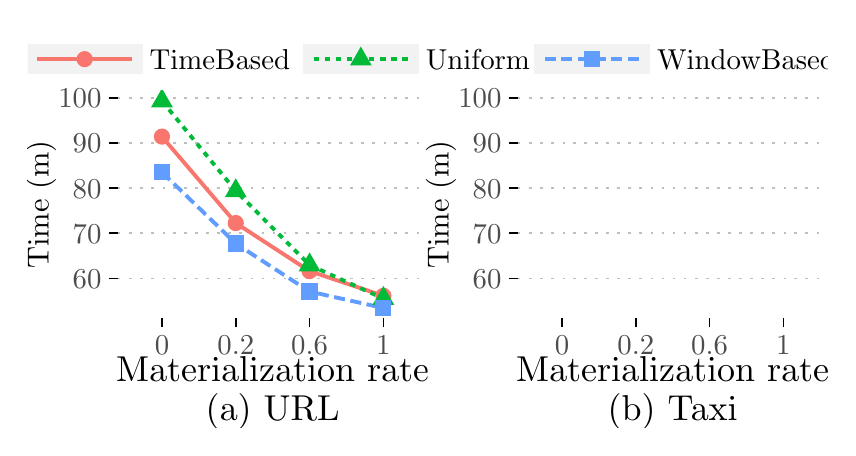
\begin{tikzpicture}[x=1pt,y=1pt]
\definecolor{fillColor}{RGB}{255,255,255}
\path[use as bounding box,fill=fillColor,fill opacity=0.00] (0,0) rectangle (289.08,144.54);
\begin{scope}
\path[clip] (  0.00,  0.00) rectangle (289.08,144.54);
\definecolor{fillColor}{RGB}{255,255,255}

\path[fill=fillColor] (-10.79,121.78) rectangle (299.87,144.54);
\end{scope}
\begin{scope}
\path[clip] (  0.00,  0.00) rectangle (289.08,144.54);
\definecolor{drawColor}{RGB}{255,255,255}
\definecolor{fillColor}{gray}{0.95}

\path[draw=drawColor,line width= 0.6pt,line join=round,line cap=round,fill=fillColor] ( -0.76,127.47) rectangle ( 41.92,138.85);
\end{scope}
\begin{scope}
\path[clip] (  0.00,  0.00) rectangle (289.08,144.54);
\definecolor{drawColor}{RGB}{248,118,109}

\path[draw=drawColor,line width= 1.4pt,line join=round] (  3.50,133.16) -- ( 37.65,133.16);
\end{scope}
\begin{scope}
\path[clip] (  0.00,  0.00) rectangle (289.08,144.54);
\definecolor{fillColor}{RGB}{248,118,109}

\path[fill=fillColor] ( 20.58,133.16) circle (  2.93);
\end{scope}
\begin{scope}
\path[clip] (  0.00,  0.00) rectangle (289.08,144.54);
\definecolor{drawColor}{RGB}{255,255,255}
\definecolor{fillColor}{gray}{0.95}

\path[draw=drawColor,line width= 0.6pt,line join=round,line cap=round,fill=fillColor] ( 99.05,127.47) rectangle (141.73,138.85);
\end{scope}
\begin{scope}
\path[clip] (  0.00,  0.00) rectangle (289.08,144.54);
\definecolor{drawColor}{RGB}{0,186,56}

\path[draw=drawColor,line width= 1.4pt,dash pattern=on 2pt off 2pt ,line join=round] (103.32,133.16) -- (137.46,133.16);
\end{scope}
\begin{scope}
\path[clip] (  0.00,  0.00) rectangle (289.08,144.54);
\definecolor{fillColor}{RGB}{0,186,56}

\path[fill=fillColor] (120.39,137.71) --
	(124.33,130.88) --
	(116.45,130.88) --
	cycle;
\end{scope}
\begin{scope}
\path[clip] (  0.00,  0.00) rectangle (289.08,144.54);
\definecolor{drawColor}{RGB}{255,255,255}
\definecolor{fillColor}{gray}{0.95}

\path[draw=drawColor,line width= 0.6pt,line join=round,line cap=round,fill=fillColor] (182.61,127.47) rectangle (225.28,138.85);
\end{scope}
\begin{scope}
\path[clip] (  0.00,  0.00) rectangle (289.08,144.54);
\definecolor{drawColor}{RGB}{97,156,255}

\path[draw=drawColor,line width= 1.4pt,dash pattern=on 4pt off 2pt ,line join=round] (186.87,133.16) -- (221.02,133.16);
\end{scope}
\begin{scope}
\path[clip] (  0.00,  0.00) rectangle (289.08,144.54);
\definecolor{fillColor}{RGB}{97,156,255}

\path[fill=fillColor] (201.02,130.23) --
	(206.87,130.23) --
	(206.87,136.08) --
	(201.02,136.08) --
	cycle;
\end{scope}
\begin{scope}
\path[clip] (  0.00,  0.00) rectangle (289.08,144.54);
\definecolor{drawColor}{RGB}{0,0,0}

\node[text=drawColor,anchor=base west,inner sep=0pt, outer sep=0pt, scale=  1.04] at ( 44.08,129.58) {TimeBased};
\end{scope}
\begin{scope}
\path[clip] (  0.00,  0.00) rectangle (289.08,144.54);
\definecolor{drawColor}{RGB}{0,0,0}

\node[text=drawColor,anchor=base west,inner sep=0pt, outer sep=0pt, scale=  1.04] at (143.90,129.58) {Uniform};
\end{scope}
\begin{scope}
\path[clip] (  0.00,  0.00) rectangle (289.08,144.54);
\definecolor{drawColor}{RGB}{0,0,0}

\node[text=drawColor,anchor=base west,inner sep=0pt, outer sep=0pt, scale=  1.04] at (227.45,129.58) {WindowBased};
\end{scope}
\begin{scope}
\path[clip] (  0.00,  0.00) rectangle (144.54,121.78);
\definecolor{drawColor}{RGB}{255,255,255}
\definecolor{fillColor}{RGB}{255,255,255}

\path[draw=drawColor,line width= 0.6pt,line join=round,line cap=round,fill=fillColor] (  0.00,  0.00) rectangle (144.54,121.78);
\end{scope}
\begin{scope}
\path[clip] ( 32.52, 39.50) rectangle (144.54,121.78);
\definecolor{fillColor}{RGB}{255,255,255}

\path[fill=fillColor] ( 32.52, 39.50) rectangle (144.54,121.78);
\definecolor{drawColor}{RGB}{255,255,255}

\path[draw=drawColor,line width= 0.3pt,line join=round] ( 32.52, 45.78) --
	(144.54, 45.78);

\path[draw=drawColor,line width= 0.3pt,line join=round] ( 32.52, 62.09) --
	(144.54, 62.09);

\path[draw=drawColor,line width= 0.3pt,line join=round] ( 32.52, 78.41) --
	(144.54, 78.41);

\path[draw=drawColor,line width= 0.3pt,line join=round] ( 32.52, 94.73) --
	(144.54, 94.73);

\path[draw=drawColor,line width= 0.3pt,line join=round] ( 32.52,111.04) --
	(144.54,111.04);
\definecolor{drawColor}{RGB}{190,190,190}

\path[draw=drawColor,line width= 0.6pt,dash pattern=on 1pt off 3pt ,line join=round] ( 32.52, 53.94) --
	(144.54, 53.94);

\path[draw=drawColor,line width= 0.6pt,dash pattern=on 1pt off 3pt ,line join=round] ( 32.52, 70.25) --
	(144.54, 70.25);

\path[draw=drawColor,line width= 0.6pt,dash pattern=on 1pt off 3pt ,line join=round] ( 32.52, 86.57) --
	(144.54, 86.57);

\path[draw=drawColor,line width= 0.6pt,dash pattern=on 1pt off 3pt ,line join=round] ( 32.52,102.89) --
	(144.54,102.89);

\path[draw=drawColor,line width= 0.6pt,dash pattern=on 1pt off 3pt ,line join=round] ( 32.52,119.20) --
	(144.54,119.20);
\definecolor{drawColor}{RGB}{255,255,255}

\path[draw=drawColor,line width= 0.6pt,line join=round] ( 48.52, 39.50) --
	( 48.52,121.78);

\path[draw=drawColor,line width= 0.6pt,line join=round] ( 75.19, 39.50) --
	( 75.19,121.78);

\path[draw=drawColor,line width= 0.6pt,line join=round] (101.86, 39.50) --
	(101.86,121.78);

\path[draw=drawColor,line width= 0.6pt,line join=round] (128.54, 39.50) --
	(128.54,121.78);
\definecolor{drawColor}{RGB}{248,118,109}

\path[draw=drawColor,line width= 1.4pt,line join=round] ( 48.52,105.17) --
	( 75.19, 73.94) --
	(101.86, 56.57) --
	(128.54, 47.64);
\definecolor{drawColor}{RGB}{0,186,56}

\path[draw=drawColor,line width= 1.4pt,dash pattern=on 2pt off 2pt ,line join=round] ( 48.52,118.04) --
	( 75.19, 85.56) --
	(101.86, 58.77) --
	(128.54, 46.65);
\definecolor{drawColor}{RGB}{97,156,255}

\path[draw=drawColor,line width= 1.4pt,dash pattern=on 4pt off 2pt ,line join=round] ( 48.52, 92.31) --
	( 75.19, 66.53) --
	(101.86, 49.19) --
	(128.54, 43.24);
\definecolor{fillColor}{RGB}{248,118,109}

\path[fill=fillColor] ( 48.52,105.17) circle (  2.93);

\path[fill=fillColor] ( 75.19, 73.94) circle (  2.93);

\path[fill=fillColor] (101.86, 56.57) circle (  2.93);

\path[fill=fillColor] (128.54, 47.64) circle (  2.93);
\definecolor{fillColor}{RGB}{0,186,56}

\path[fill=fillColor] ( 48.52,122.59) --
	( 52.46,115.76) --
	( 44.58,115.76) --
	cycle;

\path[fill=fillColor] ( 75.19, 90.11) --
	( 79.13, 83.28) --
	( 71.25, 83.28) --
	cycle;

\path[fill=fillColor] (101.86, 63.32) --
	(105.80, 56.50) --
	( 97.92, 56.50) --
	cycle;

\path[fill=fillColor] (128.54, 51.20) --
	(132.48, 44.37) --
	(124.60, 44.37) --
	cycle;
\definecolor{fillColor}{RGB}{97,156,255}

\path[fill=fillColor] ( 45.59, 89.39) --
	( 51.44, 89.39) --
	( 51.44, 95.24) --
	( 45.59, 95.24) --
	cycle;

\path[fill=fillColor] ( 72.27, 63.60) --
	( 78.12, 63.60) --
	( 78.12, 69.45) --
	( 72.27, 69.45) --
	cycle;

\path[fill=fillColor] ( 98.94, 46.26) --
	(104.79, 46.26) --
	(104.79, 52.11) --
	( 98.94, 52.11) --
	cycle;

\path[fill=fillColor] (125.61, 40.31) --
	(131.46, 40.31) --
	(131.46, 46.17) --
	(125.61, 46.17) --
	cycle;
\end{scope}
\begin{scope}
\path[clip] (  0.00,  0.00) rectangle (289.08,144.54);
\definecolor{drawColor}{gray}{0.30}

\node[text=drawColor,anchor=base east,inner sep=0pt, outer sep=0pt, scale=  1.04] at ( 26.67, 50.35) {60};

\node[text=drawColor,anchor=base east,inner sep=0pt, outer sep=0pt, scale=  1.04] at ( 26.67, 66.67) {70};

\node[text=drawColor,anchor=base east,inner sep=0pt, outer sep=0pt, scale=  1.04] at ( 26.67, 82.99) {80};

\node[text=drawColor,anchor=base east,inner sep=0pt, outer sep=0pt, scale=  1.04] at ( 26.67, 99.30) {90};

\node[text=drawColor,anchor=base east,inner sep=0pt, outer sep=0pt, scale=  1.04] at ( 26.67,115.62) {100};
\end{scope}
\begin{scope}
\path[clip] (  0.00,  0.00) rectangle (289.08,144.54);
\definecolor{drawColor}{RGB}{0,0,0}

\path[draw=drawColor,line width= 0.6pt,line join=round] ( 29.27, 53.94) --
	( 32.52, 53.94);

\path[draw=drawColor,line width= 0.6pt,line join=round] ( 29.27, 70.25) --
	( 32.52, 70.25);

\path[draw=drawColor,line width= 0.6pt,line join=round] ( 29.27, 86.57) --
	( 32.52, 86.57);

\path[draw=drawColor,line width= 0.6pt,line join=round] ( 29.27,102.89) --
	( 32.52,102.89);

\path[draw=drawColor,line width= 0.6pt,line join=round] ( 29.27,119.20) --
	( 32.52,119.20);
\end{scope}
\begin{scope}
\path[clip] (  0.00,  0.00) rectangle (289.08,144.54);
\definecolor{drawColor}{RGB}{0,0,0}

\path[draw=drawColor,line width= 0.6pt,line join=round] ( 48.52, 36.25) --
	( 48.52, 39.50);

\path[draw=drawColor,line width= 0.6pt,line join=round] ( 75.19, 36.25) --
	( 75.19, 39.50);

\path[draw=drawColor,line width= 0.6pt,line join=round] (101.86, 36.25) --
	(101.86, 39.50);

\path[draw=drawColor,line width= 0.6pt,line join=round] (128.54, 36.25) --
	(128.54, 39.50);
\end{scope}
\begin{scope}
\path[clip] (  0.00,  0.00) rectangle (289.08,144.54);
\definecolor{drawColor}{gray}{0.30}

\node[text=drawColor,anchor=base,inner sep=0pt, outer sep=0pt, scale=  1.04] at ( 48.52, 26.49) {0};

\node[text=drawColor,anchor=base,inner sep=0pt, outer sep=0pt, scale=  1.04] at ( 75.19, 26.49) {0.2};

\node[text=drawColor,anchor=base,inner sep=0pt, outer sep=0pt, scale=  1.04] at (101.86, 26.49) {0.6};

\node[text=drawColor,anchor=base,inner sep=0pt, outer sep=0pt, scale=  1.04] at (128.54, 26.49) {1};
\end{scope}
\begin{scope}
\path[clip] (  0.00,  0.00) rectangle (289.08,144.54);
\definecolor{drawColor}{RGB}{0,0,0}

\node[text=drawColor,anchor=base,inner sep=0pt, outer sep=0pt, scale=  1.30] at ( 88.53, 16.53) {Materialization rate};

\node[text=drawColor,anchor=base,inner sep=0pt, outer sep=0pt, scale=  1.30] at ( 88.53,  2.49) { (a) URL};
\end{scope}
\begin{scope}
\path[clip] (  0.00,  0.00) rectangle (289.08,144.54);
\definecolor{drawColor}{RGB}{0,0,0}

\node[text=drawColor,rotate= 90.00,anchor=base,inner sep=0pt, outer sep=0pt, scale=  1.10] at (  7.58, 80.64) {Time (m)};
\end{scope}
\begin{scope}
\path[clip] (144.54,  0.00) rectangle (289.08,121.78);
\definecolor{drawColor}{RGB}{255,255,255}
\definecolor{fillColor}{RGB}{255,255,255}

\path[draw=drawColor,line width= 0.6pt,line join=round,line cap=round,fill=fillColor] (144.54,  0.00) rectangle (289.08,121.78);
\end{scope}
\begin{scope}
\path[clip] (177.06, 39.50) rectangle (289.08,121.78);
\definecolor{fillColor}{RGB}{255,255,255}

\path[fill=fillColor] (177.06, 39.50) rectangle (289.08,121.78);
\definecolor{drawColor}{RGB}{255,255,255}

\path[draw=drawColor,line width= 0.3pt,line join=round] (177.06, 45.78) --
	(289.08, 45.78);

\path[draw=drawColor,line width= 0.3pt,line join=round] (177.06, 62.09) --
	(289.08, 62.09);

\path[draw=drawColor,line width= 0.3pt,line join=round] (177.06, 78.41) --
	(289.08, 78.41);

\path[draw=drawColor,line width= 0.3pt,line join=round] (177.06, 94.73) --
	(289.08, 94.73);

\path[draw=drawColor,line width= 0.3pt,line join=round] (177.06,111.04) --
	(289.08,111.04);
\definecolor{drawColor}{RGB}{190,190,190}

\path[draw=drawColor,line width= 0.6pt,dash pattern=on 1pt off 3pt ,line join=round] (177.06, 53.94) --
	(289.08, 53.94);

\path[draw=drawColor,line width= 0.6pt,dash pattern=on 1pt off 3pt ,line join=round] (177.06, 70.25) --
	(289.08, 70.25);

\path[draw=drawColor,line width= 0.6pt,dash pattern=on 1pt off 3pt ,line join=round] (177.06, 86.57) --
	(289.08, 86.57);

\path[draw=drawColor,line width= 0.6pt,dash pattern=on 1pt off 3pt ,line join=round] (177.06,102.89) --
	(289.08,102.89);

\path[draw=drawColor,line width= 0.6pt,dash pattern=on 1pt off 3pt ,line join=round] (177.06,119.20) --
	(289.08,119.20);
\definecolor{drawColor}{RGB}{255,255,255}

\path[draw=drawColor,line width= 0.6pt,line join=round] (193.06, 39.50) --
	(193.06,121.78);

\path[draw=drawColor,line width= 0.6pt,line join=round] (219.73, 39.50) --
	(219.73,121.78);

\path[draw=drawColor,line width= 0.6pt,line join=round] (246.40, 39.50) --
	(246.40,121.78);

\path[draw=drawColor,line width= 0.6pt,line join=round] (273.08, 39.50) --
	(273.08,121.78);

\path[] (193.06,105.17) --
	(219.73, 73.94) --
	(246.40, 56.57) --
	(273.08, 47.64);

\path[] (193.06,118.04) --
	(219.73, 85.56) --
	(246.40, 58.77) --
	(273.08, 46.65);

\path[] (193.06, 92.31) --
	(219.73, 66.53) --
	(246.40, 49.19) --
	(273.08, 43.24);
\end{scope}
\begin{scope}
\path[clip] (  0.00,  0.00) rectangle (289.08,144.54);
\definecolor{drawColor}{gray}{0.30}

\node[text=drawColor,anchor=base east,inner sep=0pt, outer sep=0pt, scale=  1.04] at (171.21, 50.35) {60};

\node[text=drawColor,anchor=base east,inner sep=0pt, outer sep=0pt, scale=  1.04] at (171.21, 66.67) {70};

\node[text=drawColor,anchor=base east,inner sep=0pt, outer sep=0pt, scale=  1.04] at (171.21, 82.99) {80};

\node[text=drawColor,anchor=base east,inner sep=0pt, outer sep=0pt, scale=  1.04] at (171.21, 99.30) {90};

\node[text=drawColor,anchor=base east,inner sep=0pt, outer sep=0pt, scale=  1.04] at (171.21,115.62) {100};
\end{scope}
\begin{scope}
\path[clip] (  0.00,  0.00) rectangle (289.08,144.54);
\definecolor{drawColor}{RGB}{0,0,0}

\path[draw=drawColor,line width= 0.6pt,line join=round] (173.81, 53.94) --
	(177.06, 53.94);

\path[draw=drawColor,line width= 0.6pt,line join=round] (173.81, 70.25) --
	(177.06, 70.25);

\path[draw=drawColor,line width= 0.6pt,line join=round] (173.81, 86.57) --
	(177.06, 86.57);

\path[draw=drawColor,line width= 0.6pt,line join=round] (173.81,102.89) --
	(177.06,102.89);

\path[draw=drawColor,line width= 0.6pt,line join=round] (173.81,119.20) --
	(177.06,119.20);
\end{scope}
\begin{scope}
\path[clip] (  0.00,  0.00) rectangle (289.08,144.54);
\definecolor{drawColor}{RGB}{0,0,0}

\path[draw=drawColor,line width= 0.6pt,line join=round] (193.06, 36.25) --
	(193.06, 39.50);

\path[draw=drawColor,line width= 0.6pt,line join=round] (219.73, 36.25) --
	(219.73, 39.50);

\path[draw=drawColor,line width= 0.6pt,line join=round] (246.40, 36.25) --
	(246.40, 39.50);

\path[draw=drawColor,line width= 0.6pt,line join=round] (273.08, 36.25) --
	(273.08, 39.50);
\end{scope}
\begin{scope}
\path[clip] (  0.00,  0.00) rectangle (289.08,144.54);
\definecolor{drawColor}{gray}{0.30}

\node[text=drawColor,anchor=base,inner sep=0pt, outer sep=0pt, scale=  1.04] at (193.06, 26.49) {0};

\node[text=drawColor,anchor=base,inner sep=0pt, outer sep=0pt, scale=  1.04] at (219.73, 26.49) {0.2};

\node[text=drawColor,anchor=base,inner sep=0pt, outer sep=0pt, scale=  1.04] at (246.40, 26.49) {0.6};

\node[text=drawColor,anchor=base,inner sep=0pt, outer sep=0pt, scale=  1.04] at (273.08, 26.49) {1};
\end{scope}
\begin{scope}
\path[clip] (  0.00,  0.00) rectangle (289.08,144.54);
\definecolor{drawColor}{RGB}{0,0,0}

\node[text=drawColor,anchor=base,inner sep=0pt, outer sep=0pt, scale=  1.30] at (233.07, 16.53) {Materialization rate};

\node[text=drawColor,anchor=base,inner sep=0pt, outer sep=0pt, scale=  1.30] at (233.07,  2.49) { (b) Taxi};
\end{scope}
\begin{scope}
\path[clip] (  0.00,  0.00) rectangle (289.08,144.54);
\definecolor{drawColor}{RGB}{0,0,0}

\node[text=drawColor,rotate= 90.00,anchor=base,inner sep=0pt, outer sep=0pt, scale=  1.10] at (152.12, 80.64) {Time (m)};
\end{scope}
\end{tikzpicture}
